\subsection{Polygonal Linkages}
\begin{figure}[h]
\begin{center}

\includegraphics[scale=1]{graphics/hingeOnThreeDistinctPolygons.pdf}
\end{center} 
\caption{(a) A polygonal linkage with a non-convex polygon and two hinge points corresponding to 
three polygons.  Note that hinge points correspond to two distinct polygons.(b) Illustrating that 
two hinge points can correspond to the same boundary point of a polygon.}
\label{fig:linkage-1}
\end{figure}
%describe how it is a generalization of Linkages.
Polygonal linkages have some differences to linkages.  Polygonal linkages have a combinatorial 
structure that is graph-like.  A polyonal linkage's combinatorial structure is an ordered pair of 
sets $\left(\PP,\HH \right)$ where $\PP$ is a set of polygons and $\HH$ is a set of hinges.  
Formally, a \textit{hinge} $h\in \HH$ 
corresponds to two points on the boundary of two distinct polygons in $\PP$.  A \emph{realization} 
of a polygonal linkage is an interior-disjoint placement of 
congruent copies of the polygons in $\PP$ such that the points corresponding to each hinge are 
identified (Fig. \ref{fig:1}). This definition of realization rules well known geometric 
dissections (e.g. Fig. \ref{fig:polygonallinkage-4}).
%this is where the geometric dissection figure belongs
\begin{figure}[h]
\begin{center}
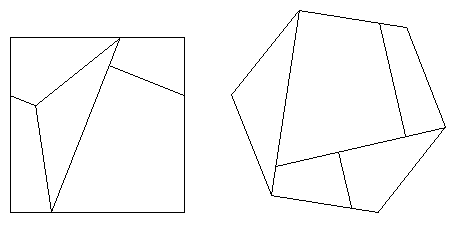
\includegraphics[scale=.25]{graphics/polygonaldissection.png}
\end{center}
\caption{Two configurations of polygonal linkage where the polygons touch on boundary segments 
instead of hinges.  These two realizations of the polygonal linkage are invalid to our definitions. 
 }
\label{fig:polygonallinkage-4}
\end{figure}
%Since polygons do not 
%exhibit a length property, a polygonal linkage does not have an edge length mapping.  


% Polygon linkages are similar to linkages.  They are an ordered pair of sets, with the exception 
% that the set of vertices become a set of hinges, $\HH$, and the set of edges become a set of 
% polygons, $\PP$.  Formally, a \textit{polygonal linkage} is an ordered pair, $G = (\HH,\PP)$,  
% comprises of a set of polygons, $\PP$, and a set of hinge points $\HH$ where each hinge $h \in \HH$ 
% corresponds to two points on the boundary of two distinct polygons in $\PP$. Mapping the linkage 
% $G$ into the plane is said to be the \textit{embedding}, i.e. $L : \HH \mapsto \bbR^{2}$.  We 
% consider a \textit{realization} of a polygonal linkage is range of $L$, i.e. $l(\HH)$.


%Foigr each hinge point $h \in \HH$, there 
%exists some subset $P \subset \PP$ with 
%at least cardinality of 2 such that for each polygon $p \in P$, $h$ corresponds to some point on 
%the boundary of $p$.  When the polygonal linkage is embedded in the plane, the hinge point is 
%where 
%the polygons of $P$ \it{kiss}.  
% show an example of polygonal linkages
\begin{figure}[h]
\begin{center}
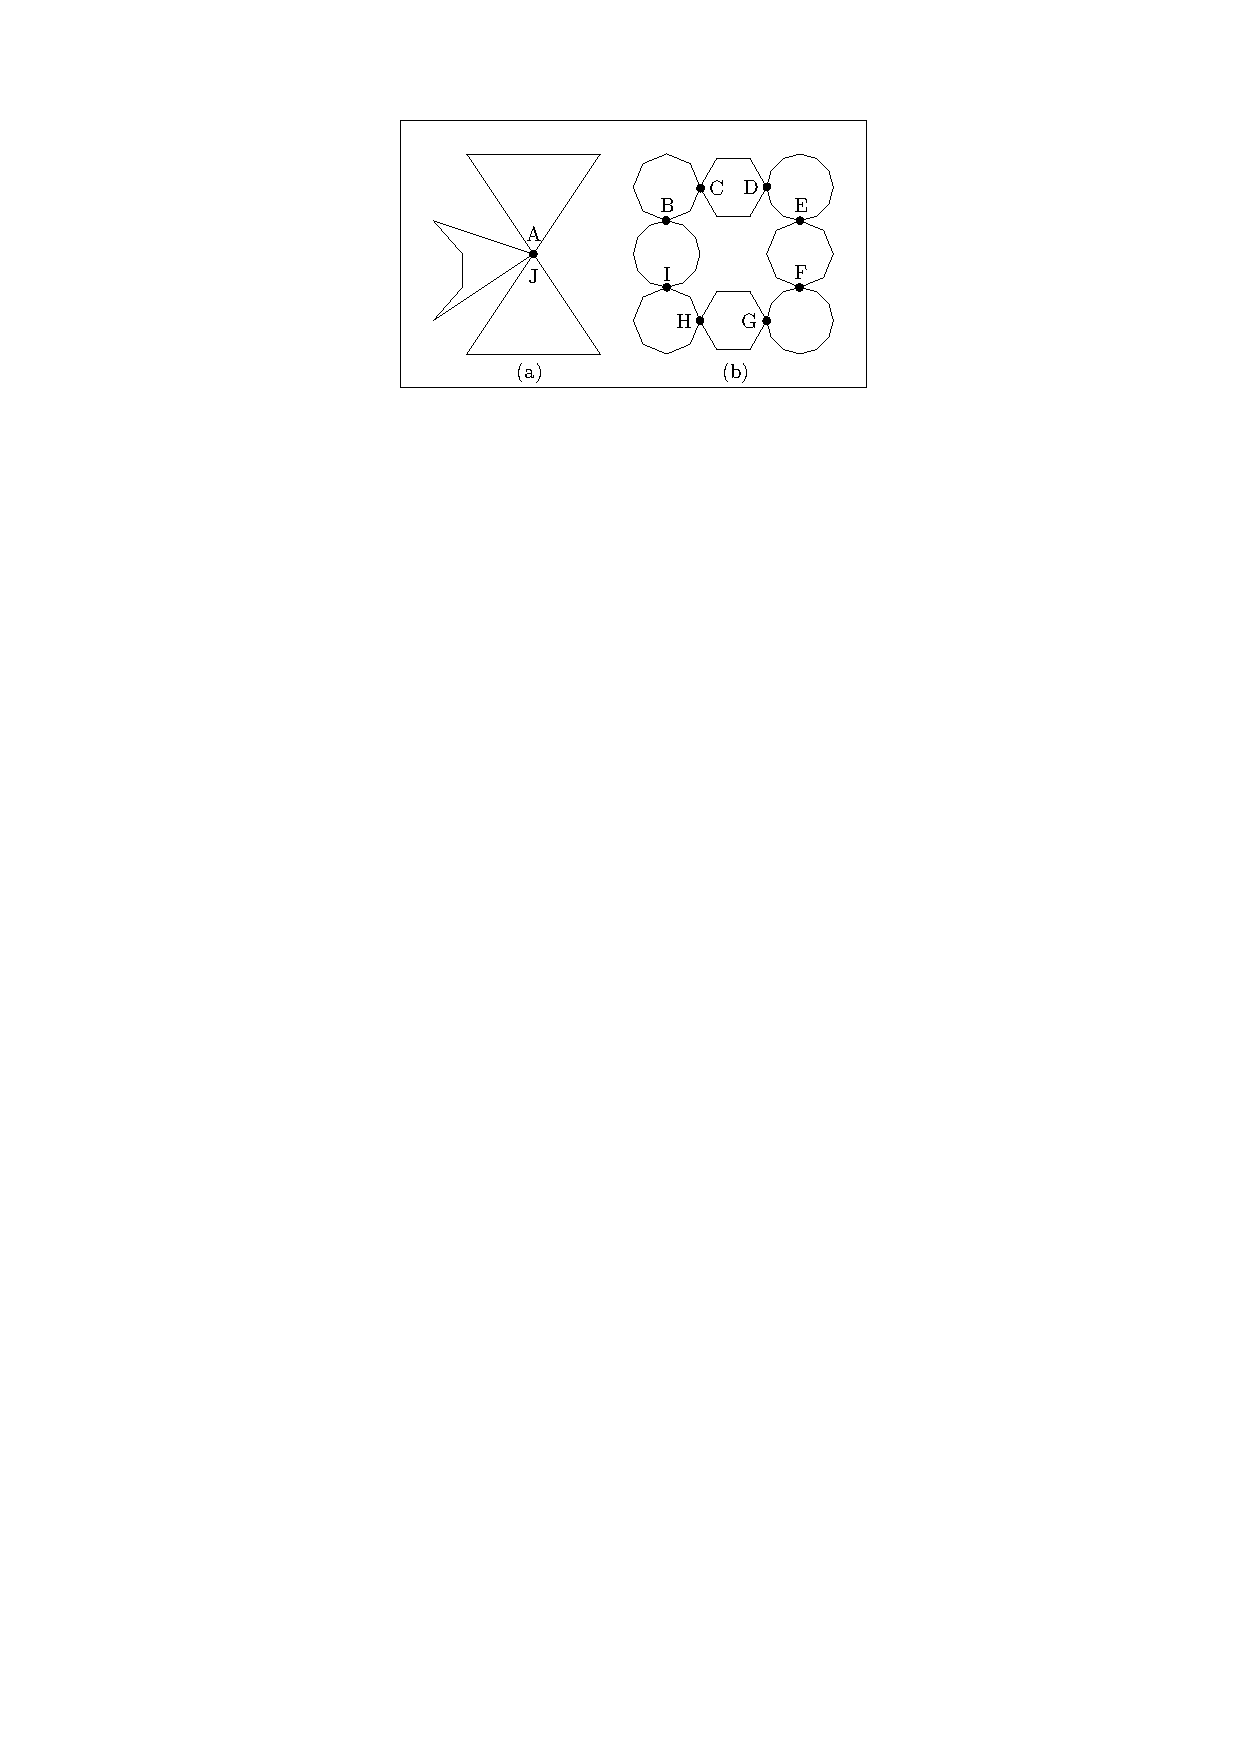
\includegraphics[scale=1]{graphics/PolygonalLinkageExamples.pdf}
\end{center} 
\caption{(a) A polygonal linkage with a non-convex polygon and a hinge point corresponding to three 
polygons.  (b) A polygonal linkage with 8 regular polygons.}
\label{fig:linkage-2}
\end{figure}
For the remainder of this thesis, we'll focus on the polygonal linkages with the following 
restrictions:
\begin{enumerate}
\item Embedded polygons must be convex, i.e. for any two embedded points $u,v \in P'$, the set:
$$\left\lbrace u  \cdot t + (1-t) \cdot v : t \in [0,1] \right\rbrace \in P'$$
 \item  Polygons can only intersect at hinge points.  No two polygons can intersect at 
their boundary or interior with the exception of possible a hinge point.  
\end{enumerate}
% Formally, we define a \it{polygonal linkage} as an ordered pair $L = (\HH,\PP)$ comprising of a 
% set of hinges, $\HH$, where each hinge $h \in \HH$ corresponds to two points on the boundary of two 
% distinct polygons. 

A difference between hinge points and embedded vertices is that two or more hinge points can be 
mapped to that same point in $\bbr^2$.  In figure (\ref{fig:linkage-2}), we illustrate that two 
hinge points can reside on the same point 
in $\bbr^2$. Figure (\ref{fig:linkage-1}) and figure (\ref{fig:linkage-3}) are examples of special 
cases that we may run into, but do not want to focus heavily on.  They are presented to the reader 
to facilitate understanding of the definitions of polygonal linkages and linkages respectively.  
Without loss of generality, for this paper, we focus on polygonal linkages that are 
equivalent to simple planar graphs.
